\chapter{Rydberg electron induced BEC losses}

\newcommand{\bogu}{\ensuremath{u^{\phantom\dagger}}\xspace}
\newcommand{\bogv}{\ensuremath{v^{\phantom\dagger}}\xspace}
\newcommand{\rhok}{\ensuremath{\rho^{\phantom\dagger}_{\veck}}\xspace}
\newcommand{\rhoq}{\ensuremath{\rho^{\phantom\dagger}_{\veck}}\xspace}
\newcommand{\rhoz}{\ensuremath{\rho^{\phantom\dagger}_{0}}\xspace}

In the s-wave approximation, the interaction between the electronic density $\rho(\vecr)=\absvsq{\Psi(\vecr)}$ in the Rydberg $n$s state and the ground state atoms is described by the interaction potential $V(\vecr)=g \rho(\vecr)$, where $g=2\pi \hbar^2 a/m_e$. Assuming a constant atomic density $n(\vecr)=V^{-1} \sum_{\vecp,\vecq} \ef{i\vecq\vecr}\aopd_{\vecp+\vecq} \aop_{\vecp}$ with annihilation operators $\aop_{\vecp}$ and quantization volume V, the interaction can be expressed as a convolution in momentum space
\begin{align}
H_\text{int} = g\intvol n(\vecr)\rho(\vecr) = \frac{g}{V} \sum_{\vecp,\vecq} \aopd_{\vecp+\vecq} \aop_{\vecp} \rhoq.
\end{align}
Neglecting constant energy shifts and two-particle excitations, we can write the interaction in terms of Bogoliubov operators $\bop_{\vecq}=\bogu_q \aop_{-\vecq} - \bogv_q \aopd_{\vecq}$ as
\begin{align}
H_\text{int}\approx\frac{g\sqrt{N_0}}{V} \sum_{\vecq\ne 0} \rho^{\phantom\dagger}_{\vecq} \big(\bogu_{q}-\bogv_{q}\big) \big(\bopd_{\vecq}+\bop_{-\vecq}\big).
\end{align}
To estimate the number of excitations induced by the presence of the Rydberg electron with lifetime $\tau=1/\gamma$, we first consider the probability to excite a certain mode with quasi momentum~$\vecq$, when a perturbation of the type $H_\text{int} \ef{-\gamma t}$ is applied. In lowest order we have
\begin{align}
P_{0\rightarrow\vecq}&=\Bigg|-\frac{i}{\hbar}\integralb{0}{\infty}{t}\ef{i\omega_{q}t-\gamma t}\braketop{\vecq}{H_\text{int}}{0}\Bigg|^2.
\end{align}
Here, $\ket{0}$ describes the many particle ground state and $\ket{\vecq}=\bopd_{\vecq}\ket{0}$ is the excited state with energy $E_{q}=\hbar\omega_{q}=\sqrt{\epsilon_{q}^2+2n_0g_c\epsilon_{q}}$, where we have used the recoil energy $\epsilon_{q}=\hbar^2 q^2/2m_\text{Rb}$, the BEC density $n_0=N_0/V$ and the atom-atom coupling constant $g_c=4\pi \hbar ^2a_{\text{Rb}}/m_{\text{Rb}}$ with the s-wave scattering length $a_{\text{Rb}}$. %The cut-off time $t_c$ is introduced to describe the field ionization process which suddenly terminates the interaction.
For the probability we find
\begin{align}
P_{0\rightarrow\vecq}=\frac{g^2 \rho_{\vecq}^2 }{V^2\hbar^2}   \integral{\omega}S(\vecq,\omega)\absvsq{C(\omega)} = \frac{g^2 \rho_{\vecq}^2}{V^2\hbar^2} N_0 \frac{\epsilon_{q}}{E_{q}} \absvsq{C(\omega_q)},
\end{align}
where $S({\vecq},\omega)=N_0 \,\epsilon_{q}/E_{q} \cdot \delta(\omega-\omega_{q})$ is the dynamic structure factor of the BEC and $C(\omega)=1/(\gamma-i \omega)$ is the Fourier transform of the exponential decay.
During the time-of-flight process, the atom-atom interactions quickly become negligible and the Bogoliubov modes are converted in to real particles. Using $N=\sum_{\veck} \aopd_{\veck}\aop_{\veck}$, we find that $\braketop{\vecq}{N}{\vecq}-\braketop{0}{N}{0} = u_{q}^2+v_{q}^2$ additional particles are in the excited state. The total number of lost atoms can now be expressed as
\begin{align}
L &= \sum_{\vecq} P_{0\rightarrow\vecq}\, (u_{q}^2+v_{q}^2).
\end{align}
Replacing the sum by an integral, we have
\begin{align}
L&= \frac{1}{2\pi^2}\frac{n_0 g^2}{\hbar^2} \integral{q} q^2\rho_q^2\,\frac{1+(q\xi)^2}{2+(q\xi)^2} \, \absvsq{C(\omega_q)}  \equiv \integral{q} P(q) (u_{q}^2+v_{q}^2)
\end{align}
where $\xi=1/\sqrt{8\pi n_0 a_{\text{Rb}}}$ is the healing length. For high principal quantum numbers we can use an asymptotic expression for the Fourier transform of the electronic density $\rho_q=J_0(q R_e/2) \operatorname{sinc}(q R_e/2)$, where we denote the electron radius by $R_e=2n^2 a_0$. We find
\begin{align} \label{eq:lostpertau2}
L/\tau^2 = \frac{2}{\pi^2}\frac{n_0 g^2}{R_e^2 \hbar^2}\integral{q} J_0(q R_e/2)^2 \sin(q R_e/2)^2 \,\frac{1+(q\xi)^2}{2+(q\xi)^2} \frac{1}{1+\omega_q^2/\gamma^2},
\end{align}
where we have separated the main dependency on the two experimentally accessible quantities on the left hand side.


To understand what kind of excitations are generated by the Rydberg electron, figure~\ref{fig:modes} shows the excitation weight $P(q)\sim P_{0\rightarrow q} q^2$ as a function of $q$. The main excitation peak is located at $q\approx 2/R_e < 1/\xi$, which lies well in the phonon regime for all principal quantum numbers investigated in the experiment.


% \begin{figure}[h]
% 	\centering
% 	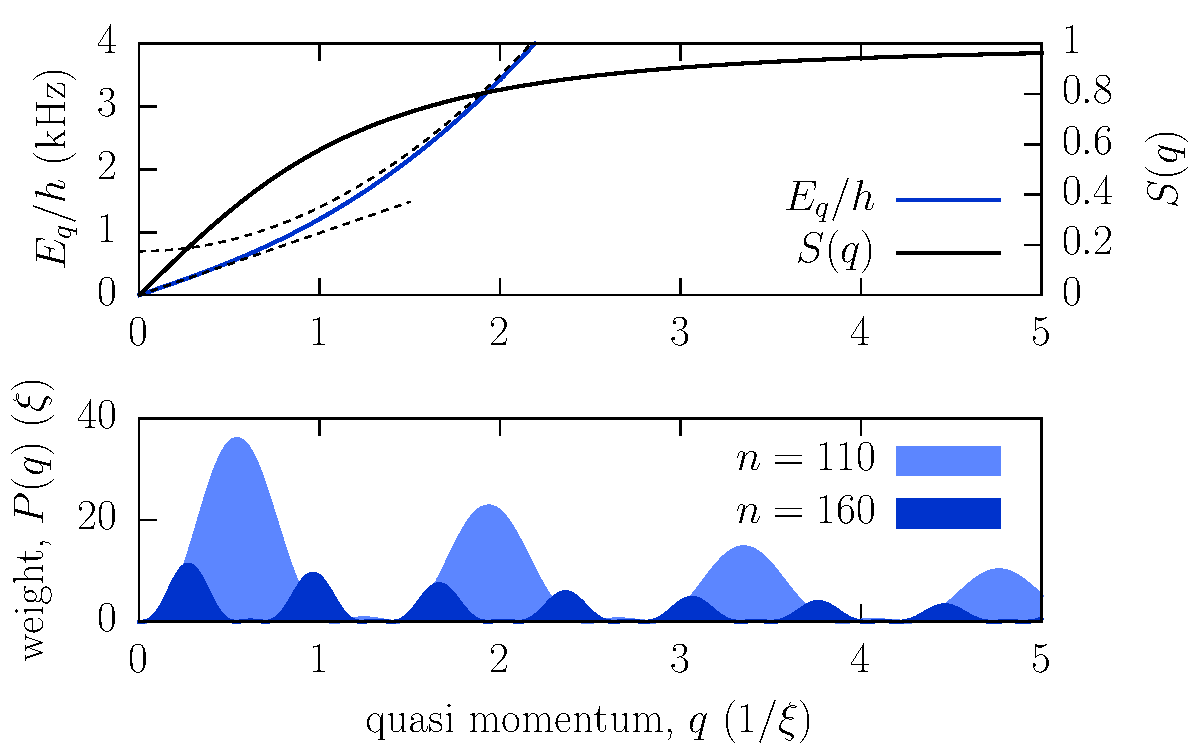
\includegraphics[width=\textwidth]{../../project_rydberg_lifetime/modes/modes}
% 	\caption{Weight of the different excitation momenta $q$ for two principal quantum numbers $n=110$ and $160$. The Bogoliubov excitation spectrum with linear and quadratic regimes is shown as a reference.}
% 	\label{fig:modes}
% \end{figure}






Some experimental details require extensions to equation \eqref{eq:lostpertau2} given above.
%\paragraph{Density:}
First, to account for density inhomogeneities due to the external potential in a simple way, we replace the BEC density $n_0$ by its mean value $n_0 \bb{1-(2R_e/5R_\rho)^2 - (R_e/5R_z)^2}$ on a sphere of radius $R_e$ centered in the middle of the cylindrical cloud with Thomas-Fermi radii $R_\rho$ and $R_z$ in radial and axial direction, respectively.

% \paragraph{Field ionization:}
Second, in the experimental sequence, the interaction between the Rydberg electron and the ground state atoms is suddenly terminated after a certain time $t_c$ at which the field ionization occurs. To account for this, the function $C(\omega)$ is modified accordingly
\begin{align}
\absvsq{C(\omega)}=\Bigg| \integralb{0}{t_c}{t}\ef{i\omega t-\gamma t} \Bigg|^2=\frac{1+\ef{-2\gamma t_c} -2 \ef{-\gamma t_c} \cos(\omega t_c)}{\gamma^2+\omega^2}
\end{align}
%\paragraph{Lower cutoff:}
The last correction concerns the way the losses are detected in the experiment. In the absorption images, excitations at small momenta cannot be distinguished from the condensate fraction due to finite momentum components in the Thomas-Fermi profile. A lower cutoff may thus be introduced in the radial $q$ integration. It turns out that this correction is negligible and almost all excitations will be detected as losses.

\section{Fourier transform of the electronic density}
The wave function of the hydrogen $n$s state is given by
\begin{align}
\Psi(r)=\frac{\ef{-\frac{r}{n}}}{\sqrt{\pi\, n^5}} \, L_{n-1}^1\!\bb{\frac{2 r}{n}}
\end{align}
where we have set $a_0=1$. The radial density distribution is given by
\begin{align}
\rho(r)=\frac{\ef{-\frac{2r}{n}}}{\pi\, n^5} \, L_{n-1}^1\!\bb{\frac{2 r}{n}}^2
\end{align}
The 3D Fourier transform for spherically symmetric functions is given by
\begin{align}
\rho_q=\frac{4\pi}{q}\integralb{0}{\infty}{r} r \sin(qr) \rho(r)
&=\frac{4}{q\,n^5}\integralb{0}{\infty}{r} r \sin(qr) \ef{-\frac{2r}{n}} \, L_{n-1}^1\!\bb{\frac{2 r}{n}}^2
\end{align}
If we replace $x=\frac{2r}{n}$, we have
\begin{align}
\rho_q=\frac{1}{q\,n^3}\integralb{0}{\infty}{x} x \sin\bb{\frac{qn}{2}x} \ef{-x} \, L_{n-1}^1\!\bb{x}^2
\end{align}
\subsection{Universal solution for $n\rightarrow\infty$}
For large $n$ we expect a universal form of $\rho_q$, if we write it as a function of the rescaled $k=2n^2 q$, where the factor $2n^2$ is just the classical electron radius in units of $a_0$. We have
\begin{align}
\rho_k = \frac{2}{k n}\integralb{0}{\infty}{x} x \sin\bb{\frac{kx}{4n}} \ef{-x} \, L_{n-1}^1\!\bb{x}^2
\end{align}

We can now expand the Laguerre polynomial as
\begin{align}
L_{n-1}^1\!\bb{x}=\sum_{\alpha=1}^{n} \binom{n}{\alpha} \frac{(-x)^{\alpha-1}}{(\alpha-1)!}
\end{align}
and then expand the square:
\begin{align}
\rho_k=\frac{2}{k n} \sum_{\alpha=1}^{n}\sum_{\beta=1}^{n} \frac{(-1)^{\alpha+\beta}}{(\alpha-1)! (\beta-1)!} \binom{n}{\alpha}\binom{n}{\beta} \integralb{0}{\infty}{x} \sin\bb{\frac{kx}{4n}} \ef{-x} x^{\alpha+\beta-1}
\end{align}
We can now evaluate
\begin{align}
    \integralb{0}{\infty}{x} \sin\bb{\frac{kx}{4n}} \ef{-x} x^{\alpha+\beta-1} &= \Im{ \integralb{0}{\infty}{x} \ef{-(1-ik /4n)x} x^{\alpha+\beta-1}} \\
    &= \Im{ \frac{(\alpha+\beta-1)!}{\bb{1-\frac{i k}{4n}}^{\alpha+\beta}} }
\end{align}
leading to
\begin{align}
    \rho_k=\frac{2}{k n} \sum_{\alpha=1}^{n}\sum_{\beta=1}^{n} (-1)^{\alpha+\beta} \frac{(\alpha+\beta-1)!}{(\alpha-1)! (\beta-1)!} \binom{n}{\alpha}\binom{n}{\beta} \Im{ \frac{1}{\bb{1-\frac{i k}{4n}}^{\alpha+\beta}} }
\end{align}
We now define $\kappa=\frac{k}{4n}$ to simplify the structure
\begin{align}
    \rho_k=\frac{1}{2n^2} \sum_{\alpha=1}^{n}\sum_{\beta=1}^{n} (-1)^{\alpha+\beta} \frac{(\alpha+\beta-1)!}{(\alpha-1)! (\beta-1)!} \binom{n}{\alpha}\binom{n}{\beta} \Im{ \frac{1}{\kappa\bb{ 1-i\kappa }^{\alpha+\beta}} }
\end{align}
We can now expand this expression into a series around $\kappa=0$. All odd orders vanish identically. For even $\nu$, the $\mathcal{O}(k^\nu)$ coefficient is given by
\begin{align}
\rho^{(\nu)}_k/\nu! &=\frac{(-1)^{\nu/2}}{2n^2 (4n)^\nu (\nu+1)!} \sum_{\alpha=1}^{n}\sum_{\beta=1}^{n} (-1)^{\alpha+\beta} \frac{(\alpha+\beta+\nu)!}{(\alpha-1)! (\beta-1)!} \binom{n}{\alpha}\binom{n}{\beta}
\end{align}
In the limit $n\rightarrow \infty$ these coefficients become
\begin{align}
\rho^{(\nu)}_k/\nu! &= \frac{(-1)^{\nu/2}}{(4n)^\nu (\nu+1)!} \binom{2\nu+1}{\nu}
\end{align}
Now the series can be summed to give the final result
\begin{align}
\rho_k &= \sum_{\nu=0,2,\dots}^\infty \frac{(-1)^{\nu/2}}{(4n)^\nu (\nu+1)!} \binom{2\nu+1}{\nu} k^\nu \\
&= J_0\bb{\frac{k}{2}}\text{sinc}\bb{\frac{k}{2}}
\end{align}
If we go back to $q$, we have
\begin{align}
\rho_q = J_0\bb{q n^2}\text{sinc}\bb{q n^2}
\end{align}

% \fig{0.5}{../../project_rydberg_lifetime/universal/universal}{universal function $\rho_k$ compared to the Fourier transform for $n=10$ and for a spherical box of equal size.}

% \fig{0.5}{../../project_rydberg_lifetime/phononfreq/phononfreq}{phonon excitation frequencies. The period of the peaks is given by $\Delta q = 2\pi/R_e = \pi/n^2 a_0$. The main peak is at $2.06/R_e$}

\subsection{Comparing to the solution for a spherical box}
The Fourier transform of a sphere with homogeneous density is given by
\begin{align}
\rho^{\text{box}}_q &= \frac{4\pi}{q}\integralb{0}{R_e}{r} r \sin(qr) \bb{\frac{4}{3} \pi R_e^3}^{-1}
\end{align}
By rescaling $q= k/R_e= k/2n^2$ we get
\begin{align}
\rho^{\text{box}}_k &= \frac{3}{k}\integralb{0}{R_e}{\bb{\frac{r}{R_e}}} \frac{r}{R_e} \sin\bb{\frac{kr}{R_e}}\\
&= \frac{3}{k} \integralb{0}{1}{x} x \sin(kx) \\
&=\frac{3}{k^3}\bb{\sin(k)-k\cos(k)}=j_0(k) + j_2(k)
\end{align}
If we compare the asymptotic behavior we find a $k^{-2}$ scaling for the box and a slightly weaker decay for the universal Fourier transform of $k^{-3/2}$

\subsection{Classical probability distribution}
% \fig{0.7}{../../project_rydberg_lifetime/universalRealSpace/universalRealSpace}{Classical probability distribution in the limit $n\rightarrow \infty$.}
By Fourier transforming the universal function $\rho_k$ back to real space we find as a function of $x=r/R_e=r/2n^2$
\begin{align}
\rho(x)=\frac{1}{32 \pi ^2 n^6}\frac{\sqrt{1+x}-\sqrt{1-x}+\sqrt{2\bb{1+\sqrt{1-x^2}}}}{ x^{3/2} \sqrt{1-x^2}}
\end{align}
which diverges at $x=0$ and the classical turning point $x=r/R_e=1$. This can be simplified to give
\begin{align}
\rho(x)=\frac{1}{16\pi^2\, n^6 \, x^{3/2} (1-x)^{1/2}}
\end{align}
It can easily be checked, that it is properly normalized
\begin{align}
4\pi \integralb{0}{R_e}{r} \rho(r/R_e) r^2 = 1
\end{align}
The radial probability function is given by
\begin{align}
P(r)=4\pi \rho(r/R_e) r^2 = \frac{2}{\pi R_e} \sqrt{\frac{r/R_e}{1-r/R_e}}
\end{align}



\subsection{Exact solution for finite $n$}
\begin{align}
\rho_q&=\frac{1}{2 n^2}\sum_{m=1}^{n} \sum_{l=1}^{n} \sum_{k=0}^{\frac{l+m-1}{2}} (-1)^{m+l+k}\binom{m+l}{2 k+1}\binom{n}{l}\binom{n}{k} \times\\
&\qquad \times\frac{ (m+l-1)! }{(l-1)!  \,(m-1)!   } \frac{\left(\frac{n q}{2}\right)^{2 k}}{\bb{1+(\frac{n q}{2})^2}^{l+m}}
\end{align}

\section{Rydberg atom induced losses}
\subsection{Interaction}
The interaction between the Rydberg electron and the ground state atoms is given by
\begin{align}
H_\text{int} = \intvol n(\vecr) \phi(\vecr,t)\qquad \phi(\vecr,t) = g\, \rho(\vecr) s(t)
\end{align}
where $n(\vecr)$ is the ground state density and $\rho(\vecr)=\absvsq{\Psi_{n00}(\vecr)}$ is the wave function of the Rydberg electron. The function $s(t)$ describes ,,pulse`` sequence. The coupling strength is given by
\begin{align}
g = \frac{2\pi\hbar^2}{m_e} a_s
\end{align}
where $a_s$ is the scattering length and $m_e\approx\mu$ is the electron mass. We can Fourier transform in space and write
\begin{align}
\phi(\vecr,t) = \frac{g}{V} \sum_{\veck} \! \ef{i\veck r} \rho_{\veck} \, s(t)
\end{align}
With $\Psi(\vecr) = V^{-1/2} \sum_k \ef{i\veck \vecr}\aop_{\veck}$, the Fourier transform of the ground state density is
\begin{align}
n_{\veck}\equiv\intvol \ef{i\veck r} n(\vecr)  = \sum_{\vecp} \aopd_{\vecp-\veck} \aop_{\vecp}
\end{align}
Then
\begin{align}
H_\text{int} &= \frac{g}{V} \integral{^3r} \! \sum_{\veck} \ef{-i\veck r}  n(\vecr)  \rho_{\veck} \,s(t)\\
&= \frac{g}{V} \sum_{\veck}   n_{-\veck} \rho_{\veck}\, s(t)\\
&= \frac{g}{V} \sum_{\vecp,\veck} \aopd_{\vecp+\veck} \aop_{\vecp} \rho_{\veck}\, s(t)
\end{align}

\subsection{Interaction in Bogoliubov operators}
Acting on the BEC wavefunction we have (neglecting the time dep.)
\begin{align}
H_\text{int} \ket{0} &= \frac{g}{V} \Bigg[ \underbrace{\underbrace{\rhoz N_0}_{\vecp=0,\veck=0} +\sum_{\veck\ne 0} \rhok\sqrt{N_0} (\bogu_k-\bogv_k) \bopd_{\veck}}_{\vecp=0 \text{ or } \vecp+\veck=0} +\\
&\qquad+ \underbrace{\sum_{\vecp\ne 0} \rhoz v_p^2-\sum_{\vecp\ne 0,\veck\ne -\vecp} \rhok \bogu_{\vecp+\veck}\bogv_{\vecp} \bopd_{\vecp+\veck}\bopd_{-\vecp}}_{\vecp\ne 0 \text{ and }\vecp+\veck\ne 0} \Bigg] \ket{0}
\end{align}
With $\rho_0=1$, the energy shift is given by
\begin{align}
\braketop{0}{H_\text{int}}{0} = \frac{g}{V} \bb{N_0 + \sum_{\vecp\ne 0} v_p^2} = g (n_0 + n_\text{depl}) = g n
\end{align}
Neglecting the two-particle excitations and the energy shifts we can write the interaction as
\begin{align}
H_\text{int}=\frac{g\sqrt{N_0}}{V} \sum_{\vecq\ne 0} \rho^{\phantom\dagger}_{\vecq} \big(\bogu_{\vecq}-\bogv_{\vecq}\big) \big(\bopd_{\vecq}+\bop_{-\vecq}\big)
\end{align}

\subsection{Exciting Bogoliubov modes}
The initial state is given by $\ket{\text{I}}=\ket{\text{BEC}}$. We proceed to calculate the rate to create one excitation in the condensate, so a possible final state is given by $\ket{\text{F}_{\vecq}} = \bopd_{\vecq}\ket{\text{BEC}}$. We consider
\begin{align}
\braketop{\text{F}_{\vecq}}{\aopd_{\vecp+\veck} \aop_{\vecp}}{\text{I}} = \meanv{b_{\vecq} \aopd_{\vecp+\veck} \aop_{\vecp}}= \sqrt{N_0} \,\delta_{\vecp,0} \, \delta_{\vecq,\vecp+\veck} (u_{\vecq}-v_{\vecq})
\end{align}

\subsection{Perturbation theory}
In the following, we calculate the probability for the system to end up in state $\ket{\text{F}_{\vecq}}$ if we apply a perturbation of the type $H_\text{int}$ with $s(t)=\ef{-\Gamma t}$. We are interested in transition probabilities for $t\gg \tau$:
\begin{align}
P_{0\rightarrow\vecq}&=\absvsq{-\frac{i}{\hbar}\integralb{0}{\infty}{t}\ef{i\omega_{\vecq}t}\braketop{\text{F}_{\vecq}}{H_\text{int}}{\text{I}}}\\
&=\frac{g^2 N_0}{V^2\hbar^2}\absvsq{\sum_{\vecp,\veck}\delta_{\vecp,0} \, \delta_{\vecq,\vecp+\veck} (u_{\vecq}-v_{\vecq}) \rho_{\veck}\integralb{0}{\infty}{t}\ef{i\omega_{\vecq}t}s(t)}\\
&=\frac{g^2 N_0}{V^2\hbar^2} (u_{\vecq}-v_{\vecq})^2 \rho_{\vecq}^2 s(\omega_{\vecq})^2
\end{align}
With $(u_{\vecq}-v_{\vecq})^2=\epsilon^0_{\vecq}/\epsilon_{\vecq}$ and
\begin{align}
s(\omega_{\vecq})=\frac{1}{\Gamma+i\omega_{\vecq}}
\end{align}
we find
\begin{align}
P_{0\rightarrow\vecq}&=\frac{g^2\rho_{\vecq}^2}{V^2\hbar^2}\, \underbrace{N_0\frac{\epsilon^0_{\vecq}}{\epsilon_{\vecq}} \, \frac{1}{\Gamma^2+\omega_{\vecq}^2}}_{=\integral{\omega}\frac{S(\vecq,\omega)}{\Gamma^2+\omega^2}}
\end{align}
with the dynamic structure factor $S(\vecq,\omega)=N_0 \frac{\epsilon^0_{\vecq}}{\epsilon_{\vecq}} \delta(\omega-\omega_{\vecq})$.
\subsection{Number of Bogoliubov excitations}
To calculate the total number of Bogoliubov excitations, we sum\footnote{with $\frac{1}{V}\sum_{\vecq}=\integralf{^3 q}{(2\pi)^3}$} over all $\vecq$ to get
\begin{align}
N_\text{bog}=\sum_{\vecq}P_{0\rightarrow\vecq}=\frac{4\pi n_0 g^2}{\hbar^2} \integralf{q}{(2\pi)^3} q^2\rho_{\vecq}^2\frac{\epsilon^0_{\vecq}}{\epsilon_{\vecq}} \, \frac{1}{\Gamma^2+\omega_{\vecq}^2}
\end{align}
where we have defined the BEC density $n_0=N_0/V$. We define the Rydberg electron radius $R_e=2n^2 a_0$ and the corresponding volume $V_e=\frac{4}{3}\pi R_e^3$. The number of ground state atoms inside the electronic wave function is roughly given by $N_e\equiv n_0 V_e$. Also, we define the mean electronic density by $n_e=V_e^{-1}$. Then,
\begin{align}
N_\text{bog}=\frac{2N_e}{3\pi} \frac{(n_e g)^2}{(\hbar\Gamma)^2} \times R_e^3 \integral{q} q^2\rho_{\vecq}^2\frac{\epsilon^0_{\vecq}}{\epsilon_{\vecq}} \, \frac{1}{1+\omega_{\vecq}^2/\Gamma^2}
\end{align}

%\subsection{Scaling law for large $n$}
%For large principal quantum numbers $n>100$ we can make certain assumptions. First of all, the Fourier transform of the electronic density $\rho_{\vecq}$ cuts off all values of $q$ which are much larger then $1/R_e\sim 1/(1\mu\text{m})$. The values are given for\footnote{For $n=210$, the $q$ value is given by $1/(4\mu\text{m})$, the cutoff frequency by $4\text{kHz}$ and the decay rate is $40\text{kHz}$.} $n=110$. In frequencies, this means that $\omega_{\vecq}$ much larger than $15\text{kHz}$ are cut off. The decay rate is $\Gamma \approx 200\text{kHz}$. Therefore, the frequency dependent factor is approximately equal to $1$. Also, the $\vecq$ values are in the phonon regime of the Bogoliubov spectrum since the healing length $\xi = \hbar/\sqrt{2m n g}\approx 0.3 \mu\text{m}$. This means, we can replace $\epsilon^0_{\vecq}/\epsilon_{\vecq}=\xi q/\sqrt{2}$.
%To get a scaling law, we can also replace $\rho_{\vecq}^2$ by 1 for $\vecq < 1/R_e$. In total, we have
%\begin{align}
%R_e^3 \integral{q} q^2\rho_{\vecq}^2\frac{\epsilon^0_{\vecq}}{\epsilon_{\vecq}} \, \frac{1}{1+\omega_{\vecq}^2/\Gamma^2}\approx R_e^3 \integralb{0}{R_e^{-1}}{q} \frac{\xi q^3}{\sqrt{2}}=\frac{\xi}{4\sqrt{2}R_e}
%\end{align}
%Then, the number of lost atoms is
%\begin{align}
%N_\text{bog}\approx \frac{N_e}{6\sqrt{2}\pi} \frac{(n_e g)^2}{(\hbar\Gamma)^2} \frac{\xi}{R_e}
%\end{align}
%or, alternatively
%\begin{align}
%N_\text{bog}\approx \frac{1}{8\sqrt{2}\pi^2} \frac{n_0 g^2}{\hbar^2 R_e^3} \frac{\xi}{R_e}\tau^2
%\end{align}
%Thus, we find
%\begin{align}
%N_\text{bog}/\tau^2 \sim n^{-8}
%\end{align}

%\fig{0.6}{../../project_rydberg_lifetime/losses/losses}{Scaling of quantitiy $N_\text{bog}/\tau^2$.}

\subsection{Number of lost atoms}
A Bogoliubov excitations with momentum $\vecq$ consists of real particles with momentum $\vecq$ and $-\vecq$. The number of free particles can be obtained from
\begin{align}
\braketop{\text{F}_{\vecq}}{\aopd_{\vecq}\aop_{\vecq}+\aopd_{-\vecq}\aop_{-\vecq}}{\text{F}_{\vecq}}=(u_{\vecq}^2+v_{\vecq}^2)+2v_{\vecq}^2
\end{align}
For the BEC state we find (zero temperature depletion of the condensate)
\begin{align}
\braketop{\text{BEC}}{\aopd_{\vecq}\aop_{\vecq}+\aopd_{-\vecq}\aop_{-\vecq}}{\text{BEC}}=v_{\vecq}^2+v_{\vecq}^2
\end{align}
The number of excited free particles is thus the difference of both: $u_{\vecq}^2+v_{\vecq}^2$. Therefore, the total is given by
\begin{align}
N_\text{lost} &= \sum_{\vecq} P_{0\rightarrow\vecq}\, (u_{\vecq}^2+v_{\vecq}^2)
\end{align}
With $u_{\vecq}^2+v_{\vecq}^2 = (\epsilon^0_{\vecq}+n g)/\epsilon_{\vecq}$ we have
\begin{align}
(u_{\vecq}-v_{\vecq})^2\times (u_{\vecq}^2+v_{\vecq}^2)&=\frac{\epsilon^0_{\vecq}}{\epsilon_{\vecq}} \times \frac{\epsilon^0_{\vecq}+n_0 g}{\epsilon_{\vecq}} = \frac{\epsilon^0_{\vecq}(\epsilon^0_{\vecq}+n_0 g)}{\epsilon^0_{\vecq}(\epsilon^0_{\vecq}+2n_0 g)}\\
&= \frac{1+\epsilon^0_{\vecq}/n_0 g}{2+\epsilon^0_{\vecq}/n_0 g}=\frac{1+(\xi q)^2}{2+(\xi q)^2}
\end{align}
Then, the total number of lost particles is
\begin{align}
N_\text{lost}&=\frac{1}{2\pi^2}\frac{n_0 g^2}{\hbar^2\Gamma^2}\ \integral{q} q^2\rho_q^2\,\frac{1+(\xi q)^2}{2+(\xi q)^2} \, \frac{1}{1+\omega_{q}^2/\Gamma^2}
\end{align}
We plug in the universal solution for $\rho_q=J_0(q R_e/2)\text{sinc}(q R_e/2)$ to obtain
\begin{align}
N_\text{lost}&=\frac{1}{2\pi^2} \frac{n_0 g^2}{\hbar^2\Gamma^2}\frac{4}{R_e^2} \ \integral{q} J_0(q R_e/2)^2 \sin(q R_e/2)^2 \,\frac{1+(\xi q)^2}{2+(\xi q)^2} \, \frac{1}{1+\omega_{q}^2/\Gamma^2}
\end{align}
The Bogoliubov energy is given by
\begin{align}
\omega_q=g_c n_0 \cdot \xi q \sqrt{2+(\xi q)^2}
\end{align}
with the contact interaction coupling $g_c=4\pi\hbar^2 a_\text{Rb}/m_\text{Rb}$. The healing length is given by
\begin{align}
\xi = \frac{\hbar}{\sqrt{2m n_0g}} = \frac{1}{\sqrt{8\pi n_0 a}}
\end{align}
Another form: Defining $\chi=\xi / R_e$ and $z = q R_e$, we have
\begin{align}
N_\text{lost}\gamma^2 = \frac{2}{\pi^2}\frac{n_0 g^2}{R_e^3 \hbar^2}\integral{z} J_0(z/2)^2 \sin(z/2)^2 \,\frac{1+(\chi z)^2}{2+(\chi z)^2} \frac{1}{1+\omega_{z/R_e}^2/\gamma^2}
\end{align}

% \fig{0.75}{../../project_rydberg_lifetime/losses/losses}{Lost atoms plotted as $N_\text{loss}\Gamma^2$.}

\section{Calculation of the mean density}
The Thomas-Fermi profile of a cigar shaped BEC is given by
\begin{align}
n(\rho,z) = n_0 \bb{1-\frac{\rho^2}{R_\rho^2}-\frac{z^2}{R_z^2}}
\end{align}
where $n_0$ is the peak density and $R_\rho, R_z$ are the Thomas-Fermi radii in radial and axial direction. To find the mean density within a sphere of radius $R_e$ (centered at the origin), we integrate
\begin{align}
\bar{n}(R_e)&=\frac{2\pi n_0}{\frac{4}{3} \pi R_e^3} \integralb{0}{\pi}{\theta} \integralb{0}{R_e}{r} r^2 \sin(\theta) \bb{1-\frac{r^2 \sin(\theta)^2}{R_\rho^2}-\frac{r^2 \cos(\theta)^2}{R_z^2}}\\
&= n_0 \bb{1-\frac{2}{5} \frac{R_e^2}{R_\rho^2} - \frac{1}{5} \frac{R_e^2}{R_z^2}}
\end{align}

% \fig{0.9}{../../project_rydberg_lifetime/lengthscales/lengthscales}{Comparing length scales}

\section{Fourier transform of truncated exponential decay}
The time dependence of the perturbation is given by
\begin{align}
s(t)=\ef{-\Gamma t} \theta(t_c-t)
\end{align}
where $t_c$ is the time at which the exponential is cut off. The Fourier transform is given by
\begin{align}
s(\omega)=\integralb{0}{t_c}{t} \ef{-\Gamma t+i\omega t}=\frac{1-\ef{-\Gamma t_c + i\omega t_c}}{\Gamma-i\omega}
\end{align}
The absolute square is given by
\begin{align}
\absvsq{s(\omega)}=\frac{1+\ef{-2\Gamma t_c} -2 \ef{-\Gamma t_c} \cos(\omega t_c)}{\Gamma^2+\omega^2}
\end{align}
In the limit $t_c\rightarrow \infty$ we recover $s(\omega)=(\Gamma^2+\omega^2)^{-1}$.

\section{Comparing contributions}
% \fig{0.9}{../../project_rydberg_lifetime/integrand_110/integrand_110}{Comparing length scales}
